\section{Interfaces del Sistema}

Las figuras de esta sección son capturas de la aplicación en operación, tomadas
sobre el entorno local con la pila completa levantada ---API, base de datos, cola
y cliente web---, y no maquetas. Los datos que aparecen en ellas provienen de un
conjunto de siembra preparado para la demostración; las imágenes de los vehículos
son recortes del material real capturado en el recinto.

La comparación con los wireframes del capítulo de diseño muestra tres diferencias
que conviene declarar antes de recorrer las vistas. La primera es que el panel de
monitoreo no reproduce el video con las cajas superpuestas: el sistema entrega el
evento confirmado y el recorte que lo evidencia, y no transmite el flujo al
navegador. La segunda es que la vista de padrón no se implementó, porque el
padrón de vehículos habilitados no forma parte del alcance
(Sección~\ref{sec:estado_gestion}); su lugar lo ocupa una búsqueda de incidentes
por ventana temporal. La tercera es que se añadió una vista de telemetría del
modelo que no estaba en el diseño, y que expone la latencia y la confianza
registradas por el sistema en operación.

La aplicación implementa dos temas, claro y oscuro. Las capturas corresponden al
tema oscuro, que es el que se emplea en operación nocturna.

\subsection{Acceso y autenticación}

La aplicación exige autenticación antes de mostrar cualquier dato. El acceso se
resuelve con usuario y contraseña, y la sesión se conserva en una cookie
inaccesible al código del navegador; la interfaz de programación rechaza las
solicitudes de lectura que no presenten un token válido. La Figura
\ref{fig:if_login} muestra la pantalla de acceso.

\begin{figure}[htbp]
    \centering
    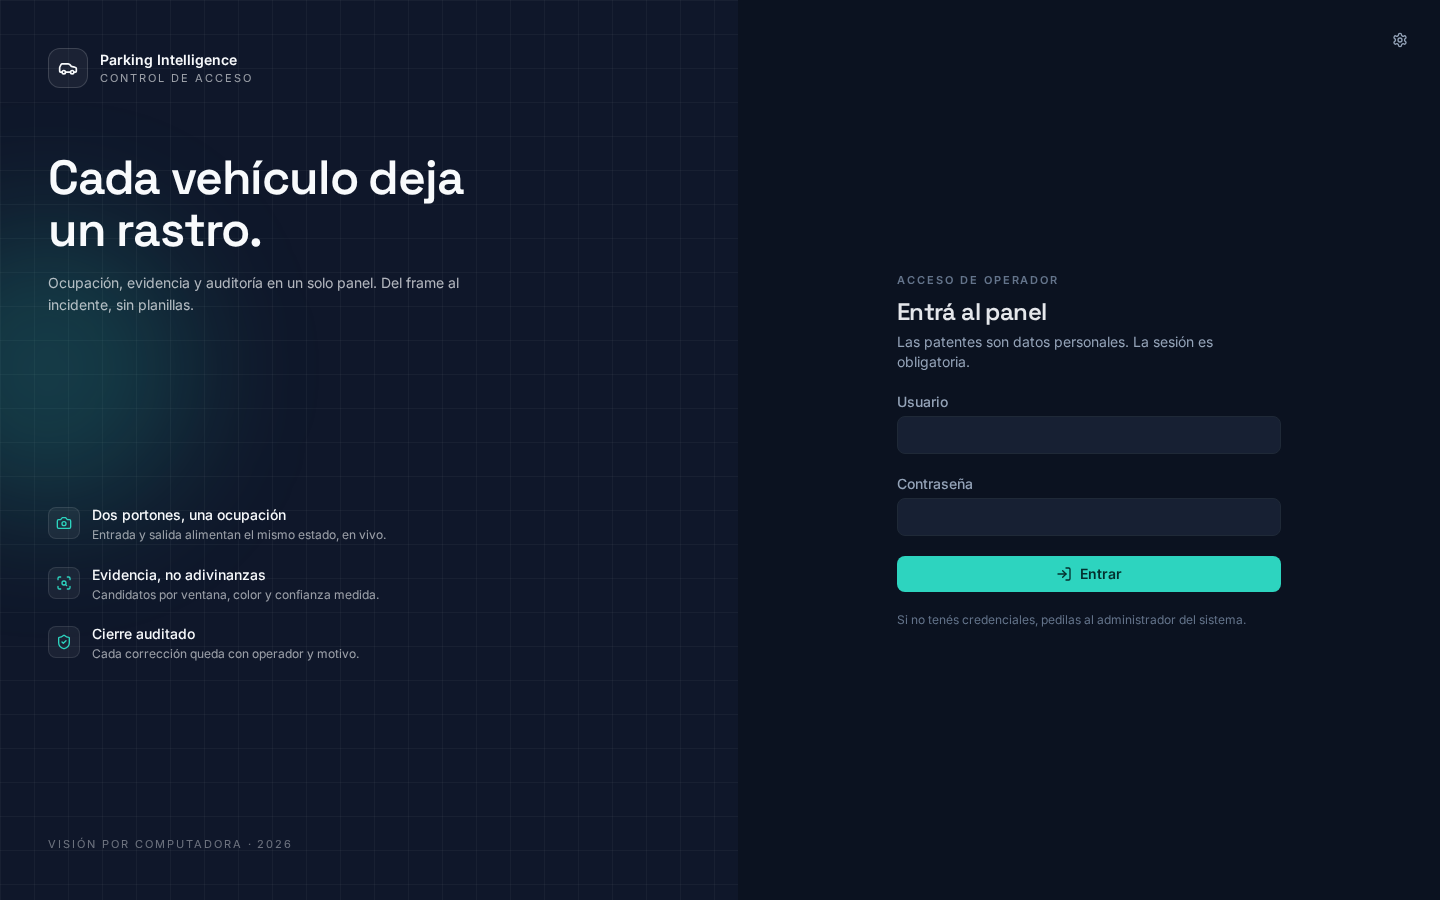
\includegraphics[width=0.92\textwidth]{fig_if_login.png}
    \caption{Pantalla de acceso a la aplicación.}
    \label{fig:if_login}
\end{figure}

\subsection{Panel de monitoreo}

El panel concentra el estado del recinto en una sola vista (Figura
\ref{fig:if_panel}). La columna izquierda presenta la ocupación como un medidor
con el número de vehículos dentro y la capacidad total; las tarjetas contiguas
resumen los ingresos del último día, la estadía promedio, la latencia del
percentil $95$ de la inferencia y la cantidad de cámaras que reportan latido.

Debajo se listan las cámaras con su puerta asignada y el instante de la última
señal, de modo que una cámara caída sea visible sin consultar registros. La lista
de vehículos activos expone, por cada sesión abierta, la matrícula, el tipo, el
color, la puerta de ingreso, el instante de entrada y el tiempo transcurrido,
junto con la acción de cierre manual. Las sesiones cuya permanencia excede el
umbral configurado se señalan con una marca de sesión huérfana: son las que
quedaron sin salida registrada y que el operador debe resolver. El panel de
eventos en vivo recibe las novedades por el canal persistente, y el gráfico
inferior presenta los ingresos de los últimos siete días.

\begin{figure}[htbp]
    \centering
    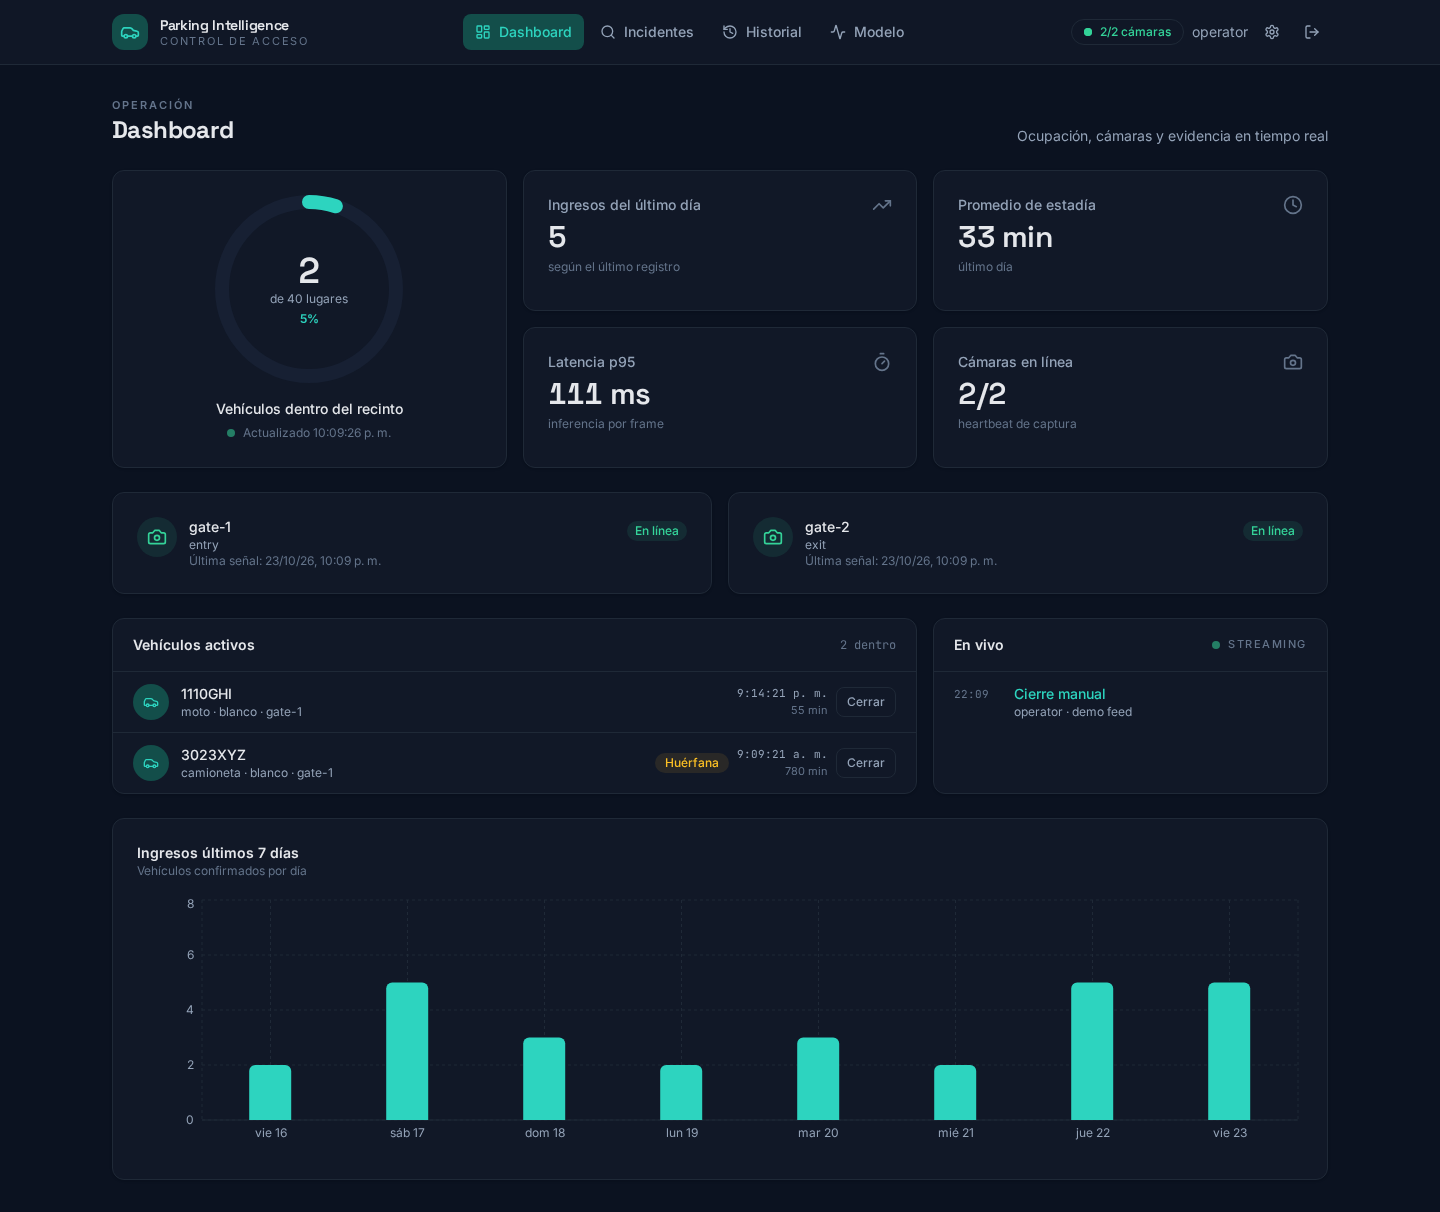
\includegraphics[width=0.95\textwidth]{fig_if_panel.png}
    \caption{Panel de monitoreo con la ocupación, el estado de las cámaras, las
    sesiones activas y el registro de eventos en vivo.}
    \label{fig:if_panel}
\end{figure}

Respecto del wireframe de la Figura~\ref{fig:wire_monitoreo}, la diferencia
principal es la ausencia del flujo de video. La decisión responde a un criterio de
costo y de arquitectura: transmitir video al navegador exige un servidor de
medios y ancho de banda continuo, mientras que el evento confirmado con su
recorte entrega la evidencia necesaria para auditar la decisión sin ese costo. La
contrapartida se asume: el operador no ve el movimiento en tiempo real, sino el
resultado de cada cruce.

\subsection{Búsqueda de incidentes y detalle del vehículo}

La vista de incidentes (Figura~\ref{fig:if_incidentes}) responde a la consulta
que motiva el sistema en la operación: qué vehículos pasaron por el acceso en una
ventana horaria determinada. El operador fija un intervalo ---por omisión, la hora
anterior y la siguiente al instante recordado--- y puede restringir por color. El
filtro de color es deliberadamente blando: incluye los vehículos cuya clasificación
está próxima al color pedido, porque el clasificador confunde tonos acromáticos y
un filtro estricto ocultaría el candidato buscado.

El resultado se presenta como una grilla de candidatos ordenada por cercanía al
instante consultado. Cada tarjeta muestra el recorte del vehículo, la matrícula
reconocida o la indicación de que no pudo leerse, el tipo y el color con su
confianza, y el instante de la observación. Los casos sin matrícula se conservan
en la lista: son precisamente los que el operador necesita revisar con la imagen.
Seleccionar una tarjeta abre el detalle del vehículo (Figura~\ref{fig:if_vehiculo}),
con el recorte de mayor tamaño disponible, los atributos con su confianza, el
identificador interno y la tabla de sesiones con ingreso, salida, duración, estado
y responsable del cierre.

\begin{figure}[htbp]
    \centering
    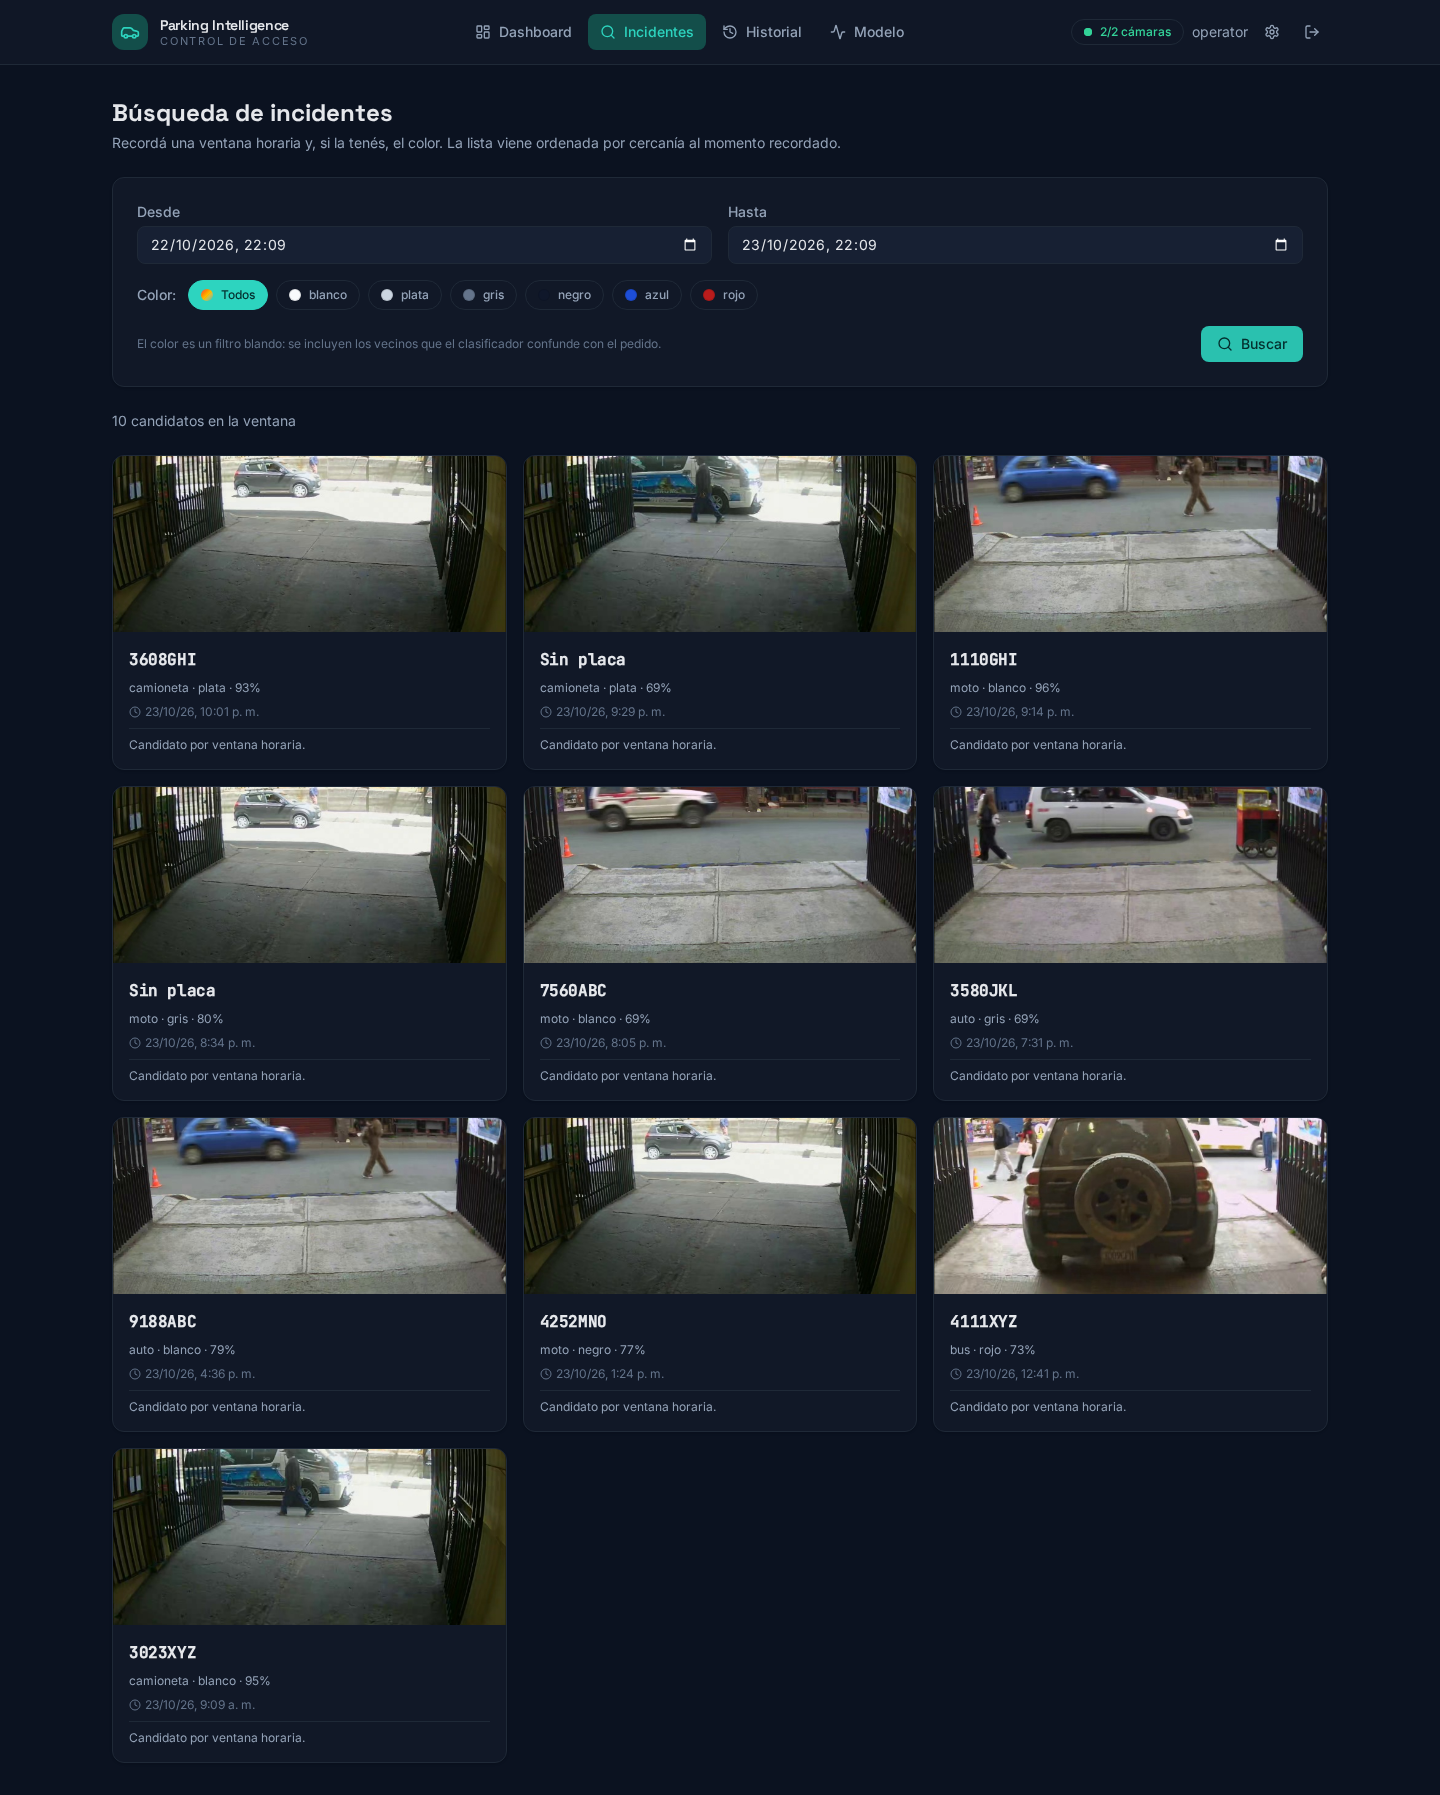
\includegraphics[width=0.95\textwidth]{fig_if_incidentes.png}
    \caption{Búsqueda de incidentes por ventana temporal y color, con los
    candidatos y su evidencia visual.}
    \label{fig:if_incidentes}
\end{figure}

\begin{figure}[htbp]
    \centering
    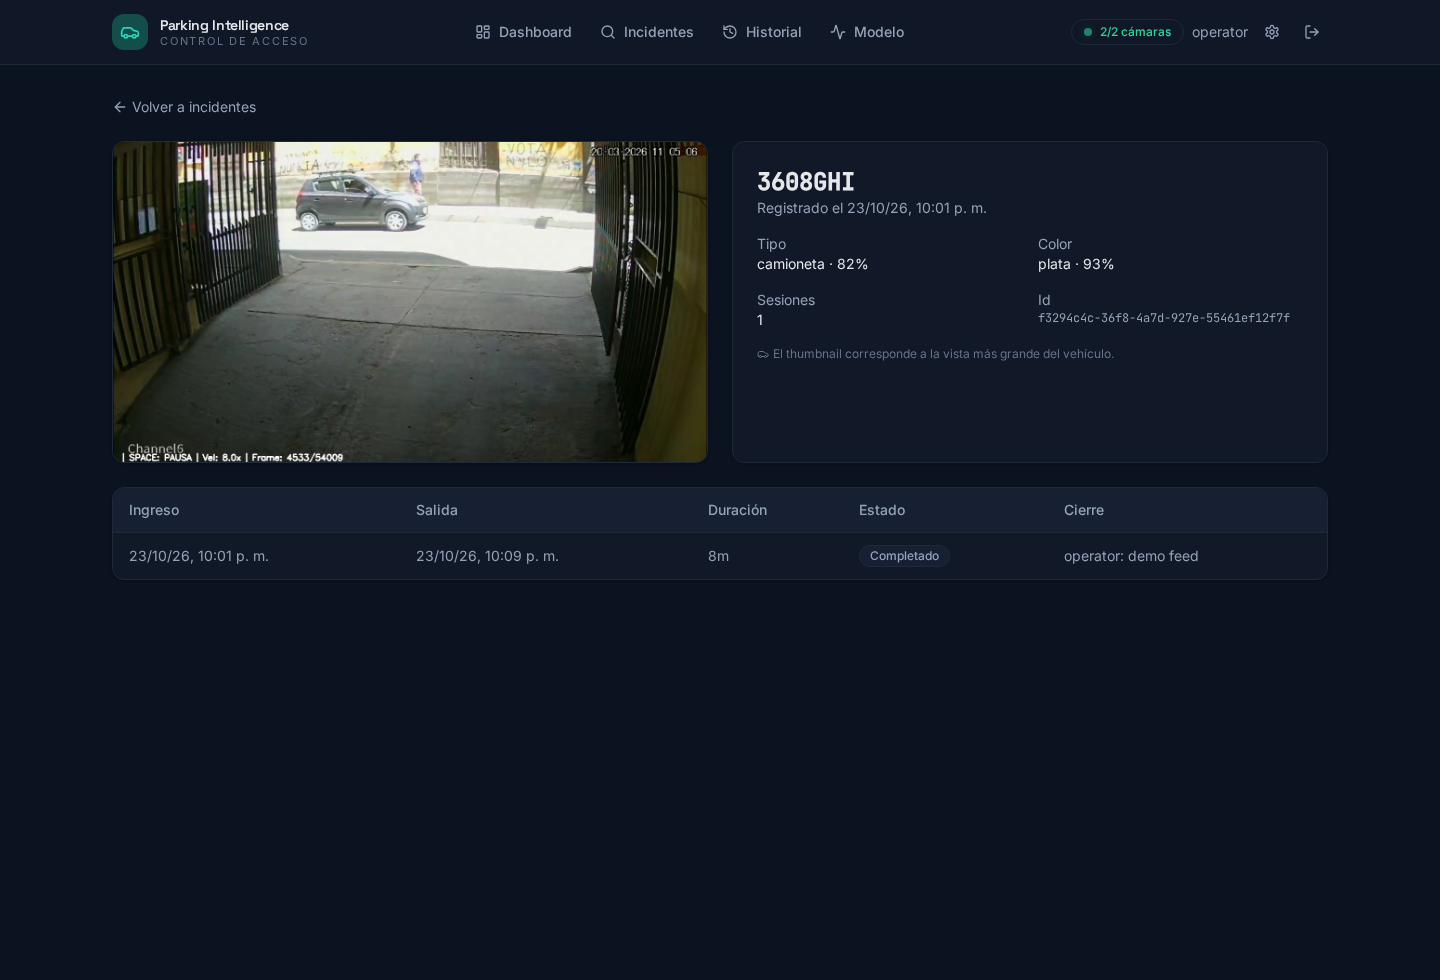
\includegraphics[width=0.95\textwidth]{fig_if_vehiculo.png}
    \caption{Detalle de un vehículo con su recorte, sus atributos y el historial
    de sesiones.}
    \label{fig:if_vehiculo}
\end{figure}

En el recorte del detalle se observa la información que el grabador superpone a la
imagen ---identificador de canal, marca temporal y contador de fotogramas---. Esa
superposición es la que el sistema anula antes de invocar al reconocimiento de
texto (Sección~\ref{subsec:ocr_crnn}): sin el enmascarado, el motor intentaría leer
caracteres que no pertenecen a la matrícula y produciría lecturas espurias.

\subsection{Historial de sesiones}

La vista de historial presenta una tabla con las sesiones registradas, ordenada de
la más reciente a la más antigua y con búsqueda por matrícula, tipo o color. Cada
fila expone la matrícula, el tipo, el color, el ingreso, la salida, la duración, el
estado de la sesión y el responsable del cierre. La consulta subyacente está
paginada por límite y desplazamiento, con un máximo de quinientos registros por
solicitud, y la vista solicita las doscientas más recientes. Su contenido es
tabular y coincide en columnas con el bloque inferior de la Figura
\ref{fig:if_vehiculo}, por lo que no se reproduce como figura independiente.

\subsection{Telemetría del modelo}

La vista de desempeño (Figura~\ref{fig:if_modelo}) no estaba prevista en el
diseño y se incorporó porque el sistema registra la latencia y la confianza de
cada evento confirmado. Presenta el total de eventos de la ventana, los modelos
que reportaron, el peor percentil $95$ de latencia y una tabla por modelo con la
confianza media y los percentiles $50$ y $95$ de la inferencia.

Su utilidad es diagnóstica: permite detectar una degradación de latencia o de
confianza sin recurrir a la base de datos. Conviene precisar su alcance para no
confundirla con una medición experimental: se alimenta de la telemetría de la
operación y está sujeta a la política de retención del sistema, de modo que
describe el comportamiento observado y no sustituye el banco comparativo por
formato de modelo que se declara pendiente en la Sección~\ref{sec:estado_gestion}.

\begin{figure}[htbp]
    \centering
    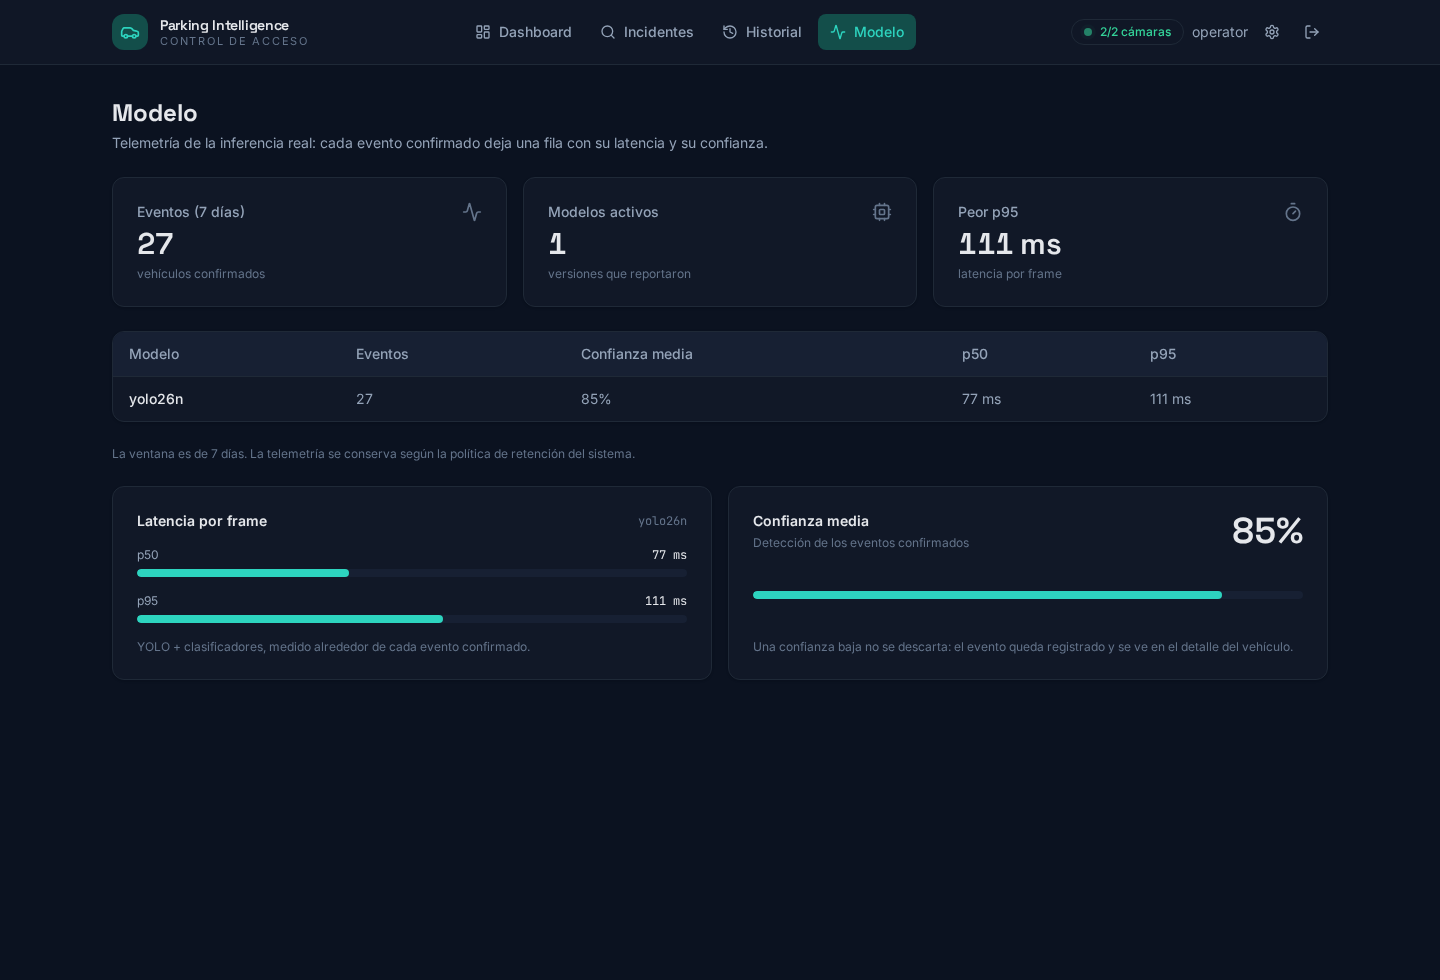
\includegraphics[width=0.95\textwidth]{fig_if_modelo.png}
    \caption{Telemetría del modelo: eventos, confianza media y latencia por
    percentil.}
    \label{fig:if_modelo}
\end{figure}

\subsection{Documentación de la interfaz de programación}

La especificación de la interfaz se genera de forma automática a partir de las
declaraciones de tipos de la aplicación y se publica en los formatos estándar de
OpenAPI. El documento resultante describe diecisiete rutas y trece esquemas de
datos, e incluye para cada operación sus parámetros, su cuerpo de solicitud, sus
respuestas y los códigos de error previstos. Al derivarse del mismo código que se
ejecuta, no puede desincronizarse de la implementación: un cambio en la firma de
un recurso se refleja en la especificación en el siguiente arranque.

La especificación no se reproduce como figura porque su valor probatorio está en
el documento generado y no en su representación visual. La Tabla
\ref{tab:api_implementada} enumera las rutas, y el documento completo se obtiene
desde el propio servicio, junto con una interfaz de exploración que permite
ejecutar cada operación contra el sistema en funcionamiento.
